\documentclass[compress,10pt,aspectratio=169]{beamer}
%\setbeamertemplate{background canvas}[bottom=white,top=structure.fg!25]
%\usetheme{Hannover}
\setbeamertemplate{headline}{}
\setbeamertemplate{footline}{June 27, 2020 - SDRA}
\setbeamersize{text margin left=0.6cm}
\usepackage{appendixnumberbeamer}
\usepackage{hyperref,listings,picinpar,mathtools} % ,enumitem}
\usepackage{color}
\settowidth{\leftmargini}{\usebeamertemplate{itemize item}}
\addtolength{\leftmargini}{\labelsep}

\beamertemplatenavigationsymbolsempty

\usepackage{listings,hyperref,multicol}
\usepackage{color,cancel}

\usepackage{listings}
\usepackage{color}

\definecolor{grey}{rgb}{0.95,0.95,0.95}
\definecolor{red}{rgb}{1.0,0.0,0.0}
\definecolor{green}{rgb}{0.0,0.7,0.0}
\definecolor{blue}{rgb}{0.0,0.0,1.0}
\lstloadlanguages{bash,Java,C,C++,csh,make,sh}%%[Visual]Basic,xml}
\lstset{frame=none,basicstyle=\footnotesize,breaklines,tabsize=2,captionpos=b,prebreak={\hbox{$\rightarrow$}},postbreak={\hbox{$\hookrightarrow$}},showstringspaces=false,backgroundcolor=\color{grey}\bfseries,keywordstyle=\color{blue},commentstyle=\color{green}\textit,stringstyle=\color{red}\ttfamily,abovecaptionskip=2pt,aboveskip=0pt,belowskip=0pt,belowcaptionskip=0pt}
%\lstset{moredelim=[is][\color{red}]{_+_}{_+_}}

\graphicspath{{/home/jmfriedt/enseignement/diapason/}{/home/jmfriedt/femto/sipat/hdr/}{/home/jmfriedt/femto/sipat/}{/home/jmfriedt/femto/sipat/hdr/imec/summary_imec/}{/home/jmfriedt/femto/sipat/hdr/eftf09/}{/home/jmfriedt/femto/sipat/hdr/Presentation/Imagez/}{/home/jmfriedt/femto/sipat/hdr/fit_parabole/}{/home/jmfriedt/femto/sipat/hdr/gps_scan/}{./hdr/allan_gps/}{/home/jmfriedt/senseor/projets/lovefood/140226_freiburg/}{/home/jmfriedt/senseor/projets/lovefood/simulations/lovefood/130115_lovefood/}} % DOIT avoir / a la fin

\beamertemplatefootpagenumber

\usepackage{graphicx,verbatim,multicol}
%\usepackage[pdftex,colorlinks=true,bookmarks=true,bookmarksopen=true,pagebackref=false,breaklinks=true,pdfauthor={Jean-Michel FRIEDT}]{hyperref}

\begin{document}

\title{Quartz tuning fork stroboscopic displacement field measurement}
\author[J.-M Friedt]{J.-M Friedt\\ \ \\ 
FEMTO-ST/Time \& Frequency department \\ \ \\ jmfriedt@femto-st.fr \ \\ \ \\
slides and references at \url{jmfriedt.free.fr}}
\maketitle

\section{Introduction}
\begin{frame}[fragile]\frametitle{Quartz tuning fork}

\vspace{0.1cm}
\hspace*{7.68cm}\includegraphics[height=4.9cm]{/home/jmfriedt/enseignement/sqnx/platforms/Atmega32/diap_sem.png}
\vspace{-5.1cm}

\noindent
\begin{itemize}
\item the ``quartz'' in quartz watch
\item the time reference is given by a tuning fork
\footnote{W.E. Newell, {\em Miniaturization of tuning forks}, Science {\bf 161} (3848), 1320--1326 (1968)}
\footnote{later an atomic transition from an atom in the Cs clock} \\
vibrating at $32768=2^{15}$~Hz $\Rightarrow$ 
counter (binary\\ frequency divider) to reach 1~Hz
\item piezoelectricity as an efficient way of \\generating mechanical vibration under control\\
of an electrical signal
\item acoustic signal: compact component since \\wave velocity is shrunk by
$10^5$ with respect to\\ electromagnetic (10~km $\rightarrow$10~cm)
\item initially a single beam vibrating at a few kHz: many spurious modes + lower quality factor
\item 1960: replace a single beam with a tuning fork (Seiko Quartz Astron at 8192~Hz)
\item from an engineering perspective: tuning fork = electrical dipole with extremely high
quality factor
\item from a physicist perspective: vibrating prongs made of a piezoelectric crystal
\end{itemize}

\vspace{0.05cm}
\end{frame}

\begin{frame}[fragile]

\vspace{-.21cm}
\begin{minipage}[t]{\linewidth}
\begin{minipage}{.49\linewidth}
\begin{itemize}
\item Tuning fork fundamental mode frequency
\vspace{-0.4cm}
$$f_0\simeq 0.1615\frac{w}{L^2}\sqrt\frac{E}{\rho}$$ 
\vspace{-0.4cm}

{\footnotesize with length $L\simeq
3.36$~mm and width $w\simeq 436$~$\mu$m, Young modulus
$E\in 75:100$~GPa (anisotropic) and density $\rho\simeq 2650$~kg/m$^3$ -- 
N.A: $f_0\in [33:38]$~kHz\par}
{\tiny L. Bates {\em \& al.}, {\em Determination of the temperature dependence
of Young's modulus for stainless steel using a tuning fork}, J. Undergrad.
Res. in Physics {\bf 18} (1), 9--13 (1999)\par}
{\tiny {\bf Note:} J. Falter {\em \& al.}. {\em Calibration of quartz tuning fork spring constants ...} 
(2014): the length of the prong should be to the stress minimum $>$ geometrical length\par}
\item high $Q\simeq 70000$ (drops to 7000 in air)
\item $Q$ is defined as the stored energy/energy dissipated
during each oscillation
\item the time needed to release the stored energy is $Q/\pi$
oscillations or $Q/(\pi f)$~s @ $f=32768$~Hz
\item in an second order resonator circuit, the width at half
height of the resonance (real part of admittance) is $\delta f=f/Q$
\item low temperature coefficient
\end{itemize}
\end{minipage}
\begin{minipage}{.53\linewidth}
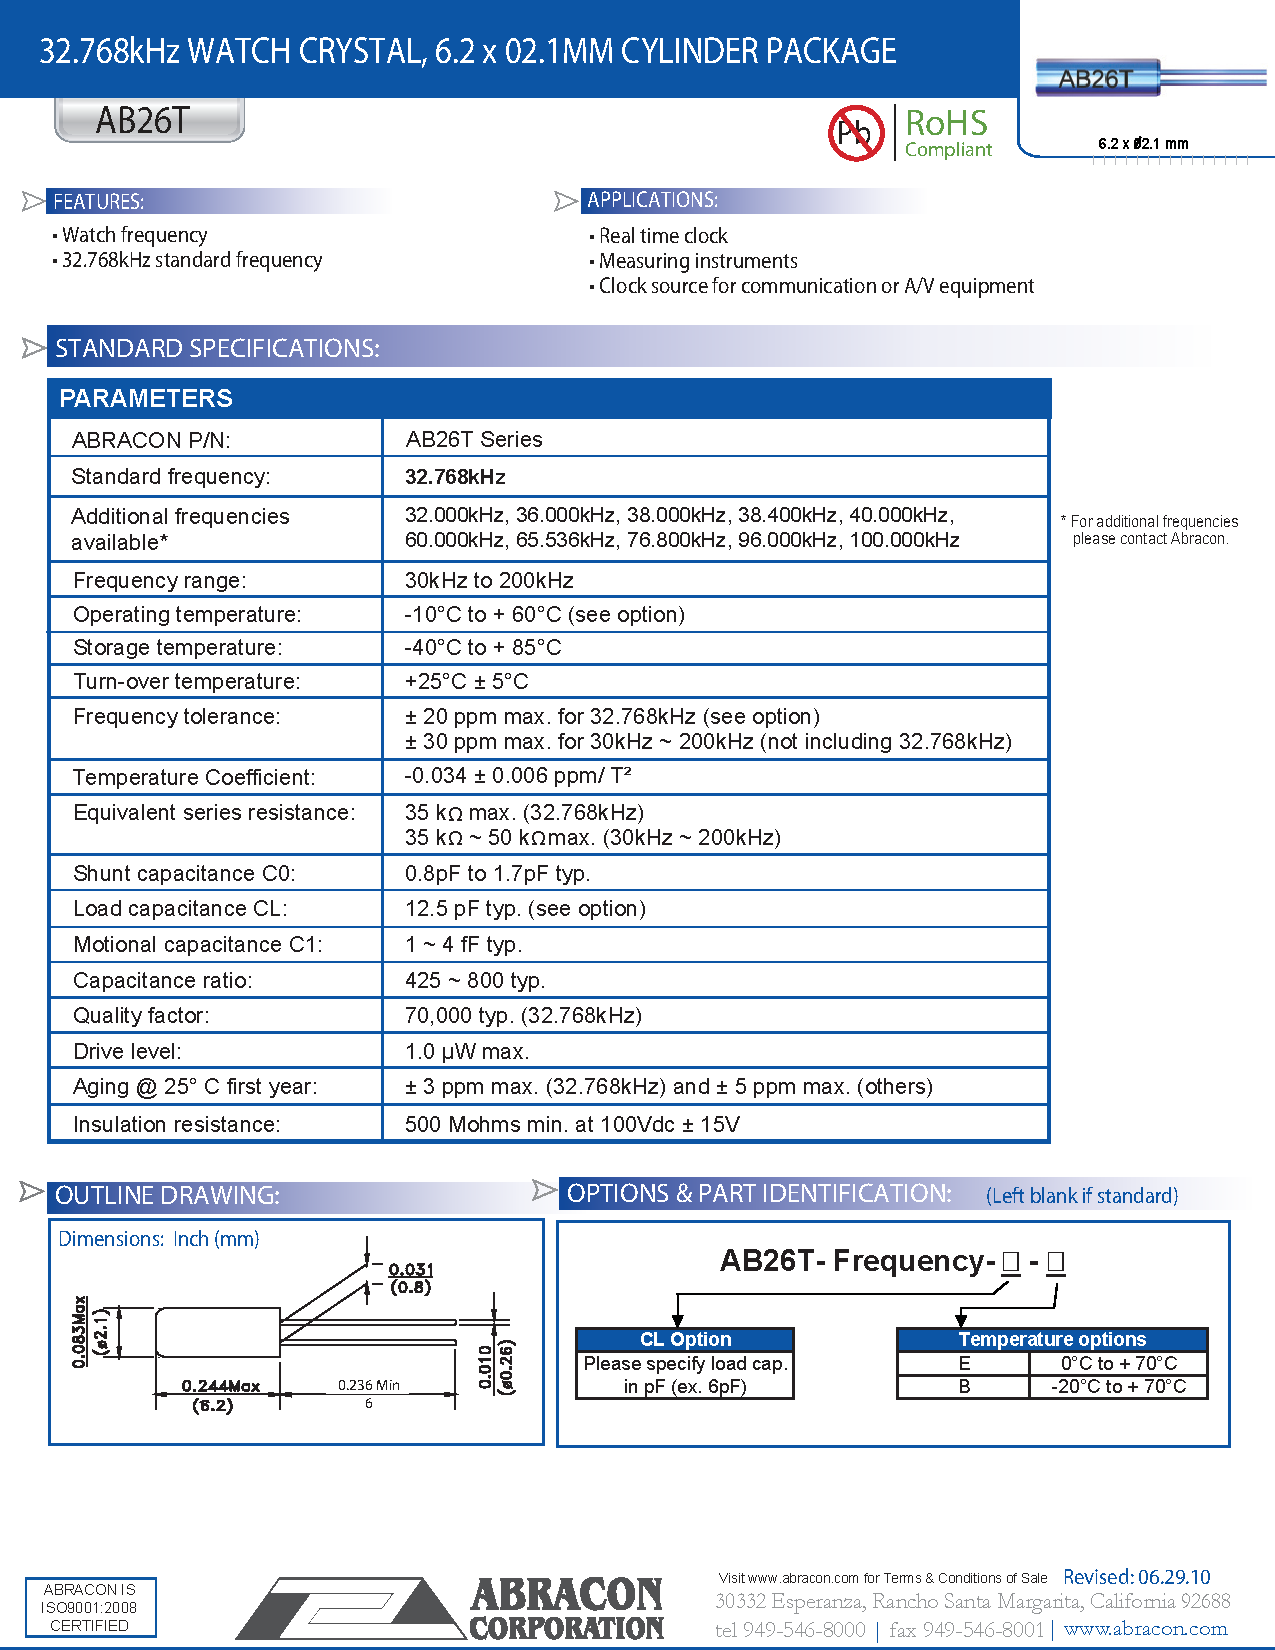
\includegraphics[width=\linewidth]{Abracon_tuning_fork_datasheet}
\end{minipage}
\end{minipage}
\end{frame}

\begin{frame}[fragile]\frametitle{Quartz tuning fork characterization}

We wish to characterize the tuning fork electrical transfer function $Y(f)$ by sweeping $f$ and monitoring
the current (measured as voltage on a load resistor)

\hfill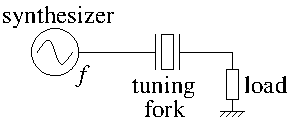
\includegraphics[width=.4\linewidth]{slide4}

Questions:
\begin{enumerate}
\item what is the frequency step $df$ at which $f$ must be swept~?
\item how long shall we wait between two steps of $df$
\end{enumerate}
\vfill
$\Rightarrow$ challenge: observe the tuning fork prong motion using a personnal computer sound
card and a commercial, off the shelf (COTS) webcam
\end{frame}

\begin{frame}[fragile]\frametitle{Sound card}

\begin{itemize}
\item Many current sound cards will exhibit $>$48~kS/s sampling rate (usually 96~kS/s or 192~kS/s)
\item Driving the 32768~Hz tuning fork with this signal is possible ...
\item ... but COTS webcams exhibit much lower framerate -- 25 or 30~fps
\item Can we ``freeze'' the prong \\motion during such long \\
(40-33~ms) exposures~?
\item Yes if the tuning fork is only \\illuminated when the prongs \\
are in the same position: \\{\bf stroboscopy}
\end{itemize}
\vspace{-2.8cm}
\hfill\includegraphics[width=.67\linewidth]{strobo}
\end{frame}

\begin{frame}[fragile]\frametitle{Stroboscopic setup}
However, illuminating for a short duration (1/10th of the period is 3~$\mu$s or 300~kHz bandwidth)
is way beyond the capability of a sound card \\
$\Rightarrow$ dedicated hardware controlled by
a stereo sound card.

\begin{itemize}
\item Pulse = convert a sine wave to a square wave and to a pulse
\item Pulse = phase shifted copies of the same sine wave
\item Phase shift = time delay = RC circuit
\item sine $\rightarrow$ Schmitt trigger (square, 2) $\rightarrow$ RC delay $\rightarrow$ Schmitt trigger (square) $\rightarrow$ \& with (2) $\rightarrow$ pulse
\end{itemize}

\only<1>{\includegraphics[width=0.597\linewidth]{fig4a_eng}
\includegraphics[width=0.38\linewidth]{fig4b}}
\only<2>{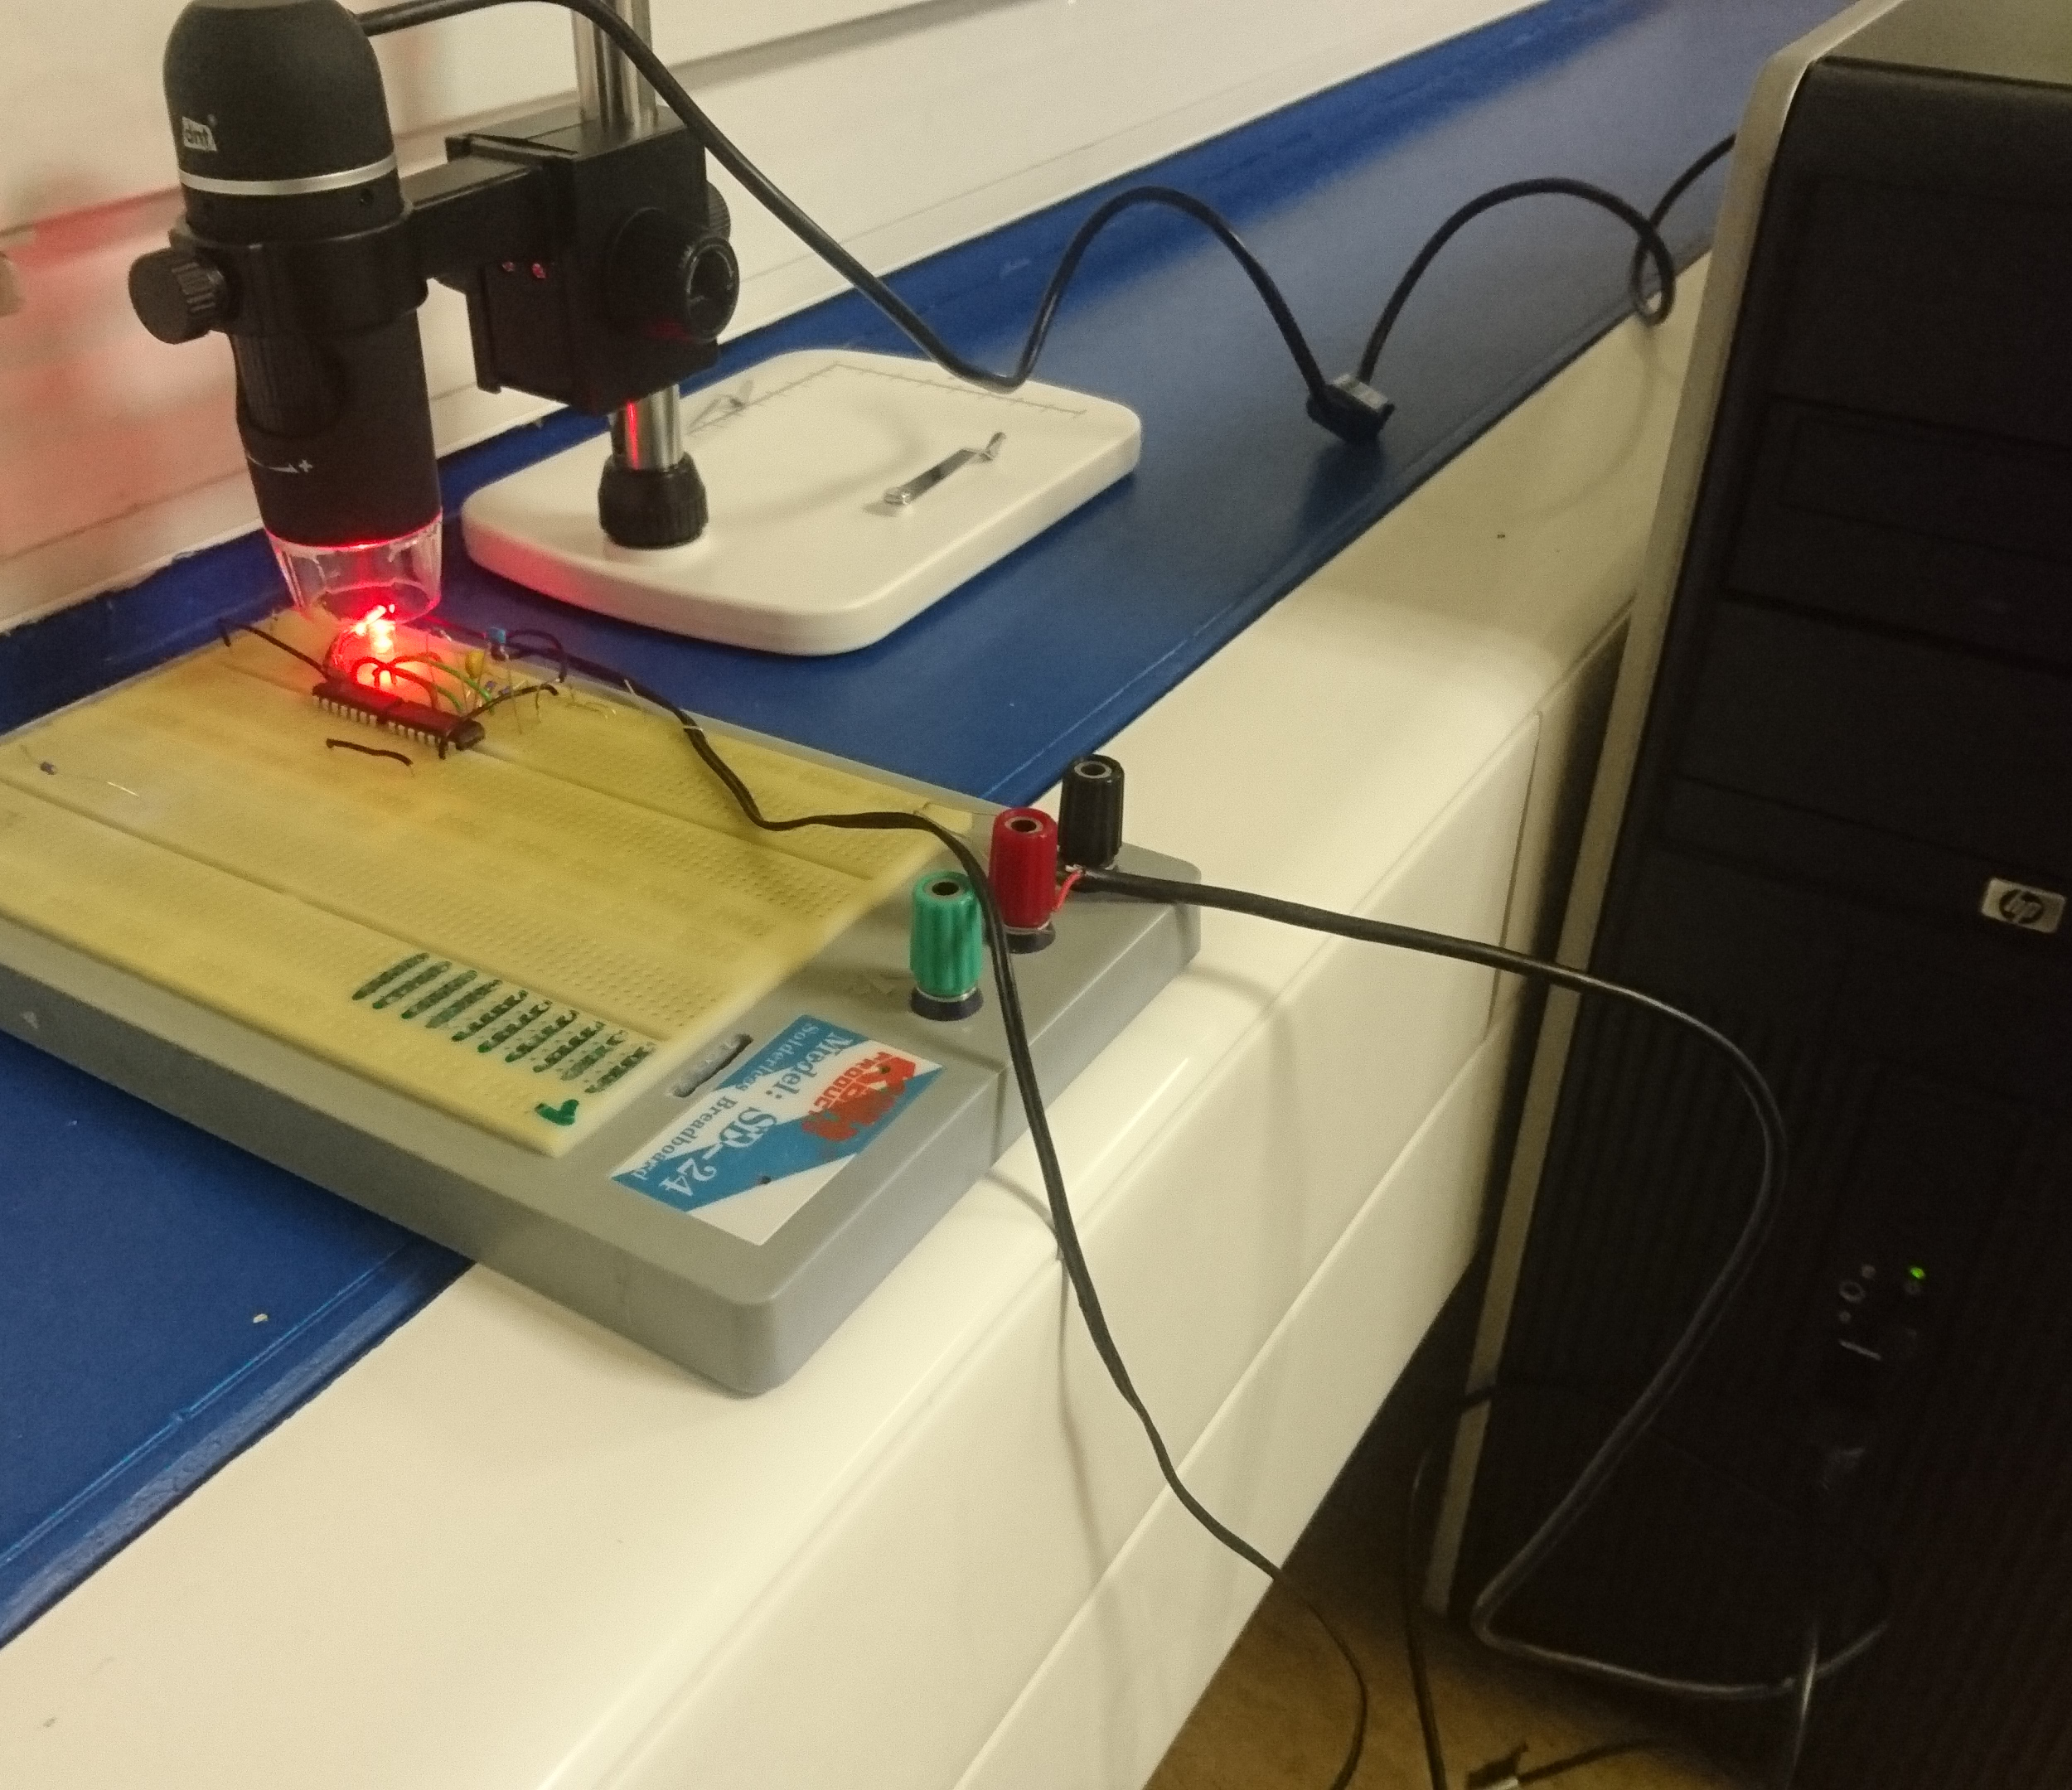
\includegraphics[width=0.48\linewidth]{DSC_2942.JPG}
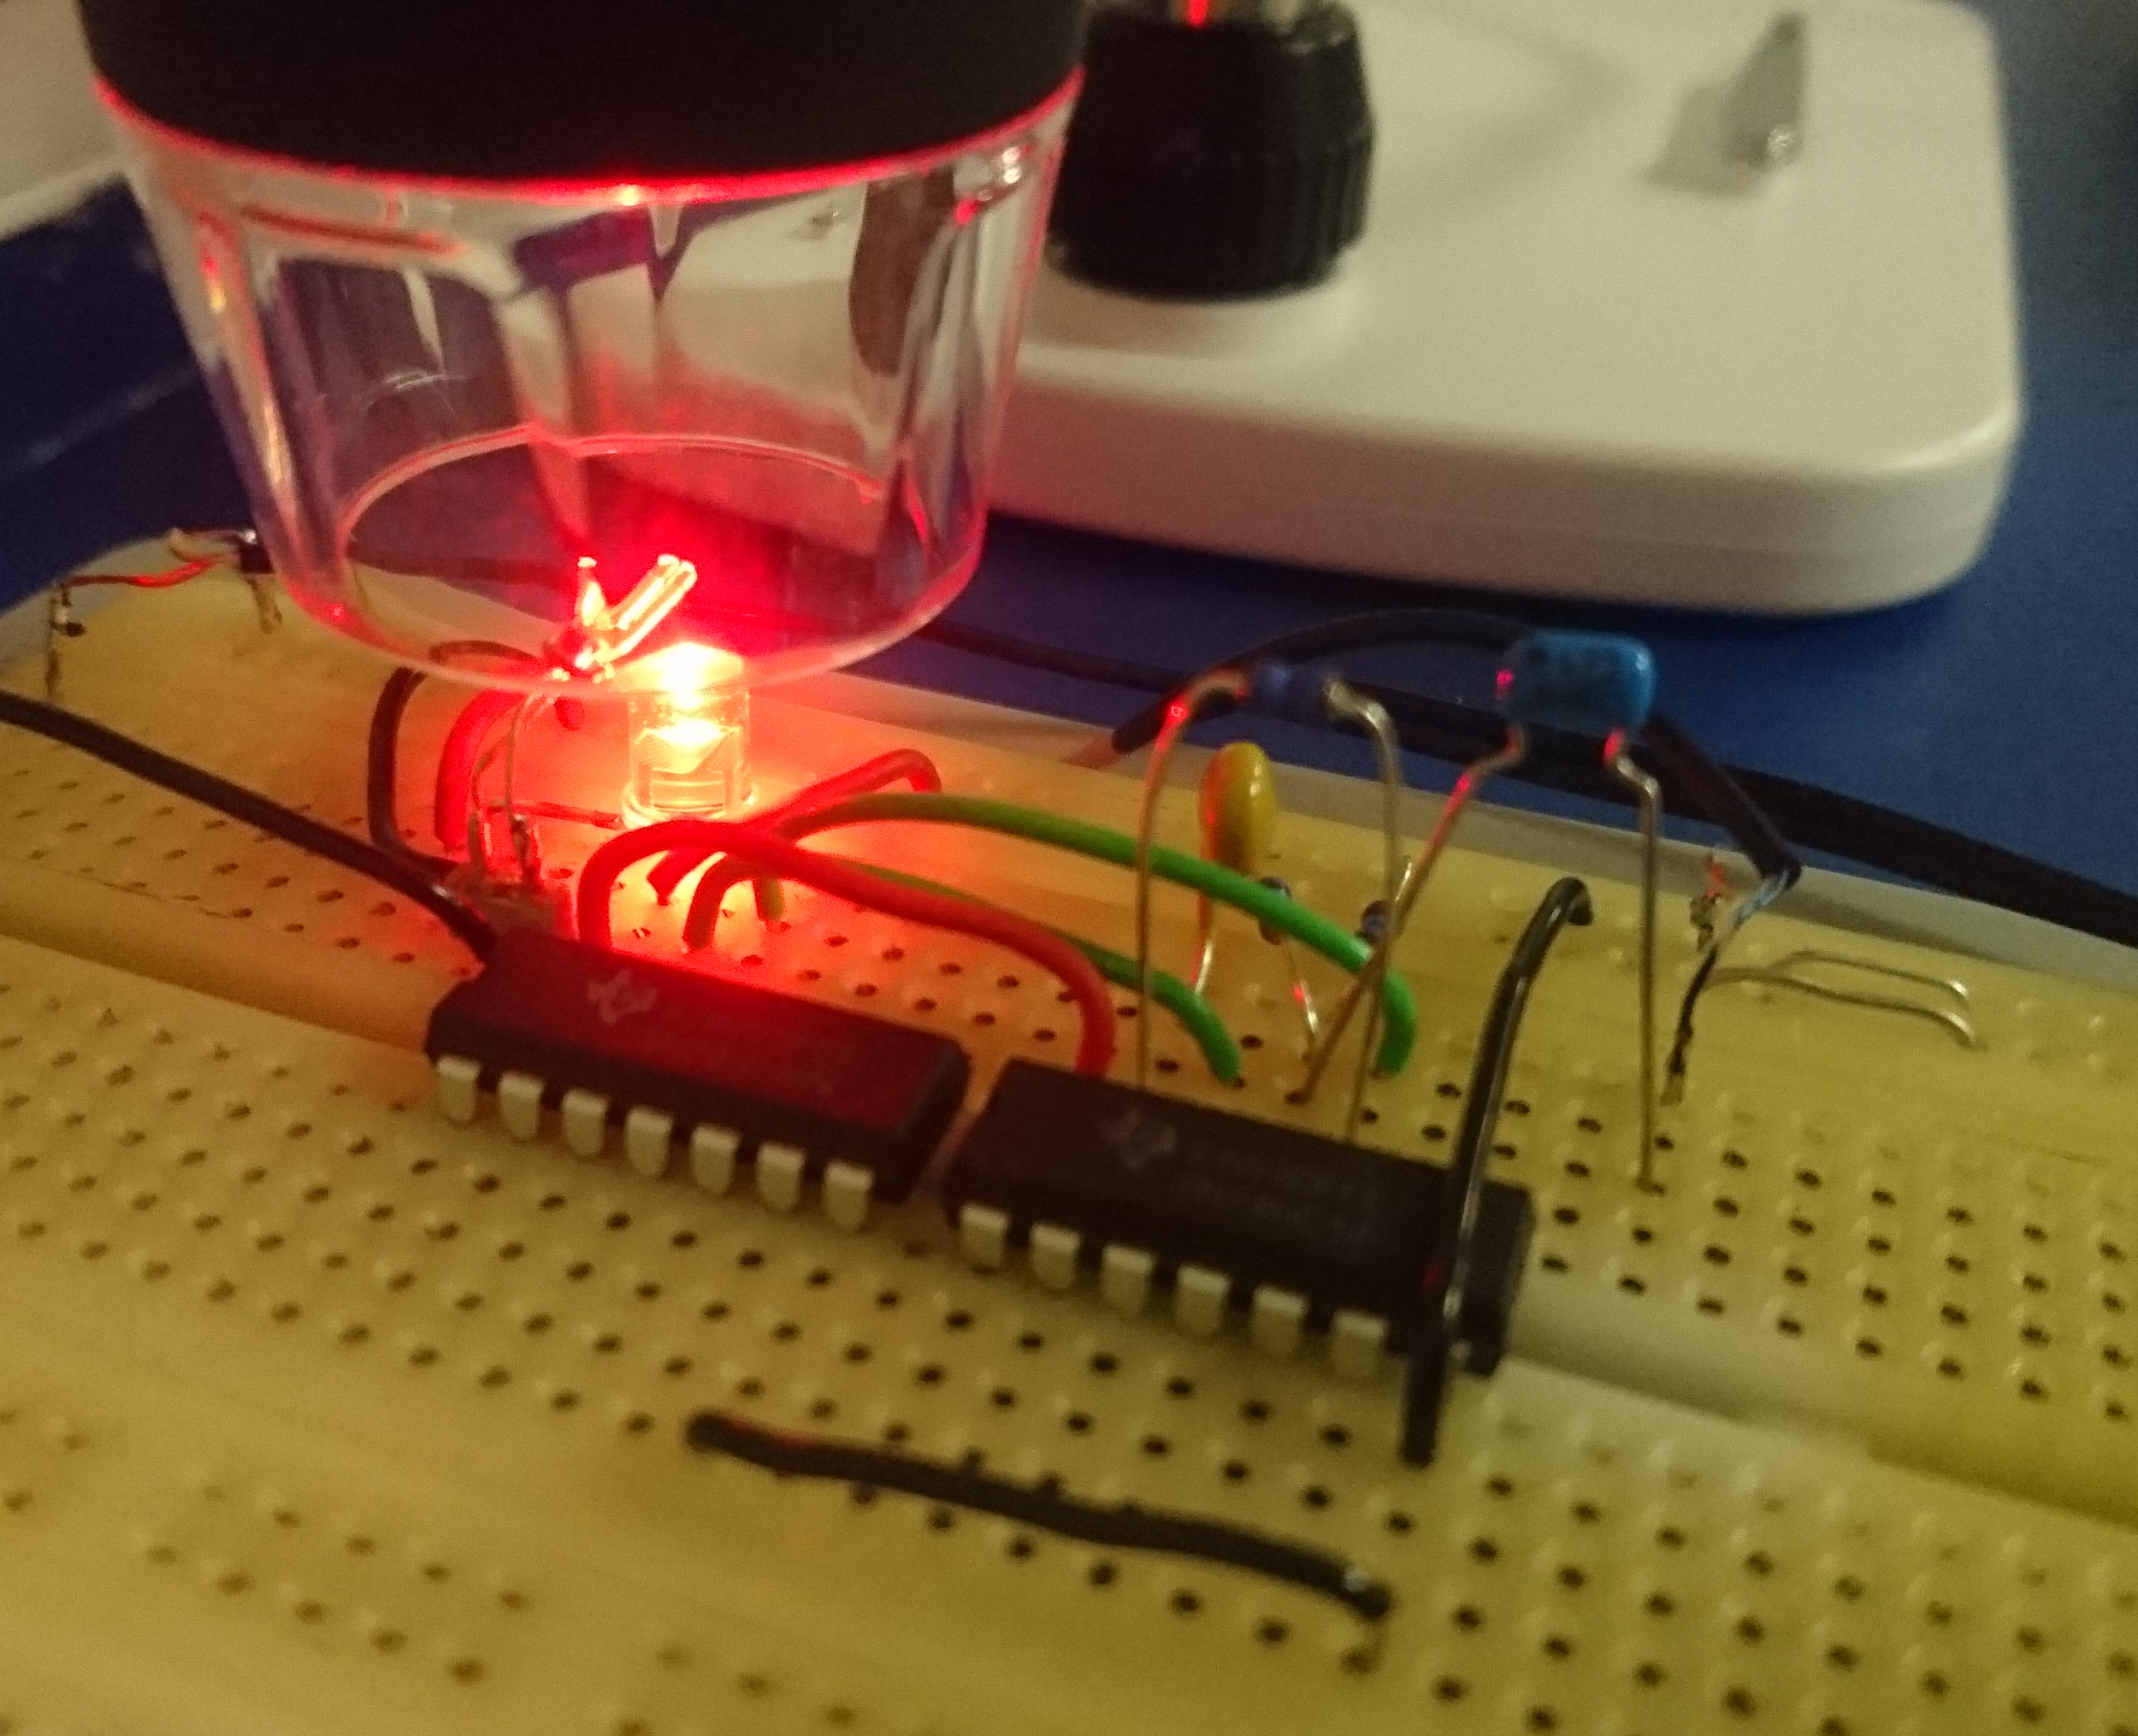
\includegraphics[width=0.51\linewidth]{DSC_2943.JPG}}
\end{frame}

\begin{frame}[fragile]\frametitle{Hardware setup: the bias T}

\begin{itemize}
\item a digital gate triggers around 1.5~V
\item sound card output is 0-mean value
\item offset the mean value without changing the AC spectral characteristics: bias T
\end{itemize}

\hfill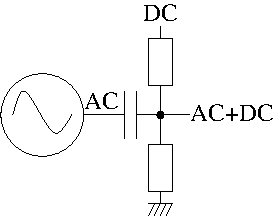
\includegraphics[width=.3\linewidth]{biasT}

\vfill {\bf Question:} considering the resistors have been selected as 1~k$\Omega$ resistances so that the current
in the voltage divider bridge is $DC/2$~mA, how do we select the capacitor value so that the bias T output
is the sum of DC+AC around 32768~Hz~?
\end{frame}

\begin{frame}[fragile]\frametitle{Image processing}

Movies (.avi format) have been recorded for various $f$ driving frequencies

\begin{enumerate}
\item Decompose each movie to a series of pictures ({\tt mplayer -vo jpeg movie.avi})
\item Select an area representative of the prong motion
\item Compute the displacement of
this area as the \\
cross-correlation maximum position between
the \\first image and the second image

\only<1>{
\vspace*{-1.52cm}
\hfill\includegraphics[width=0.47\linewidth]{fig7}
\vspace*{-1.62cm}
}

\item Repeat for all images, cross-correlating the \\$N$th image with the first
\item Display the motion of the prong
\only<2>{

\vspace*{-2.93cm}\hfill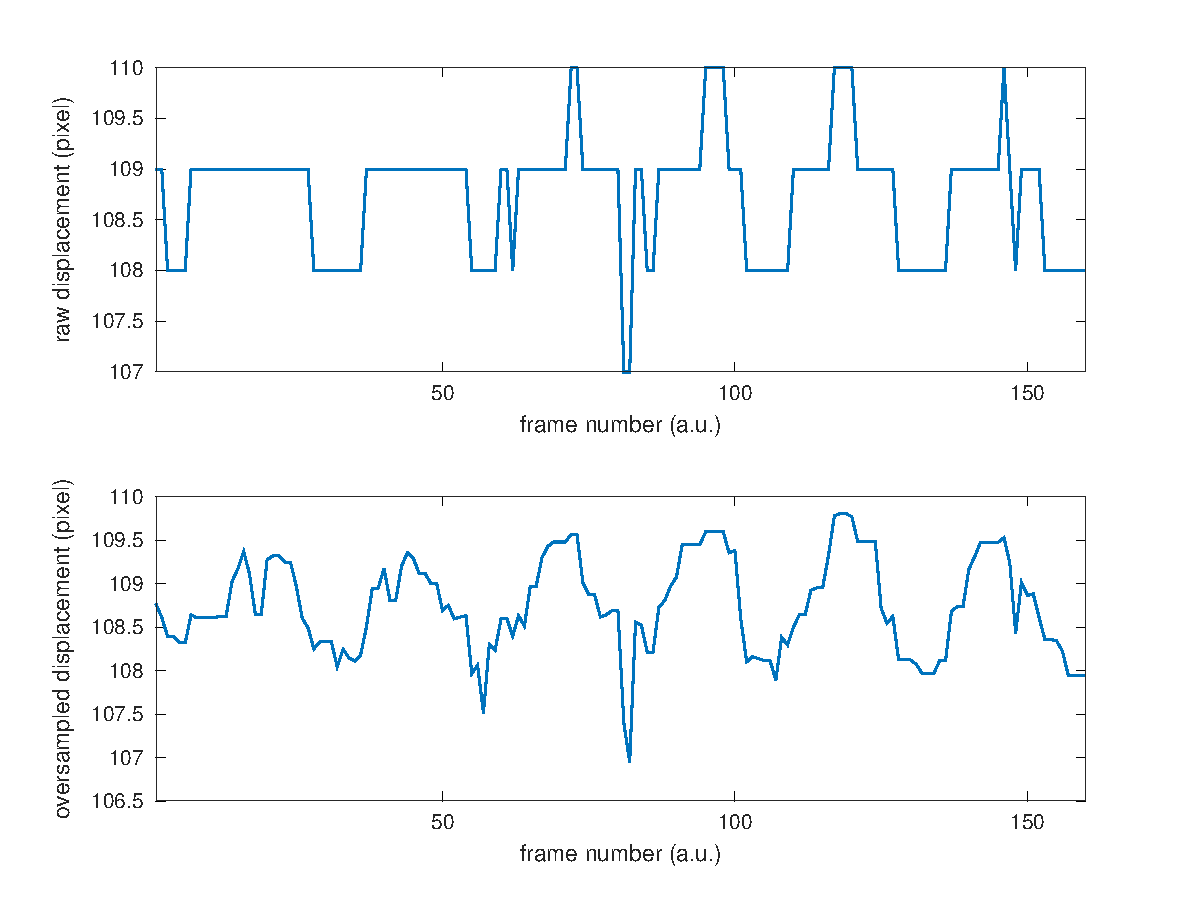
\includegraphics[width=0.49\linewidth]{oversampling.pdf}
\vspace*{-0.3cm}
}
\item Since the motion is only a few pixels, we use an \\oversampling technique of fitting the correlation 
\only<3>{\\}
maximum and identifying the position of the fit \only<3>{\\}maximum
\item Repeat for each frequency
\only<3>{

\vspace*{-4.7cm}
\hfill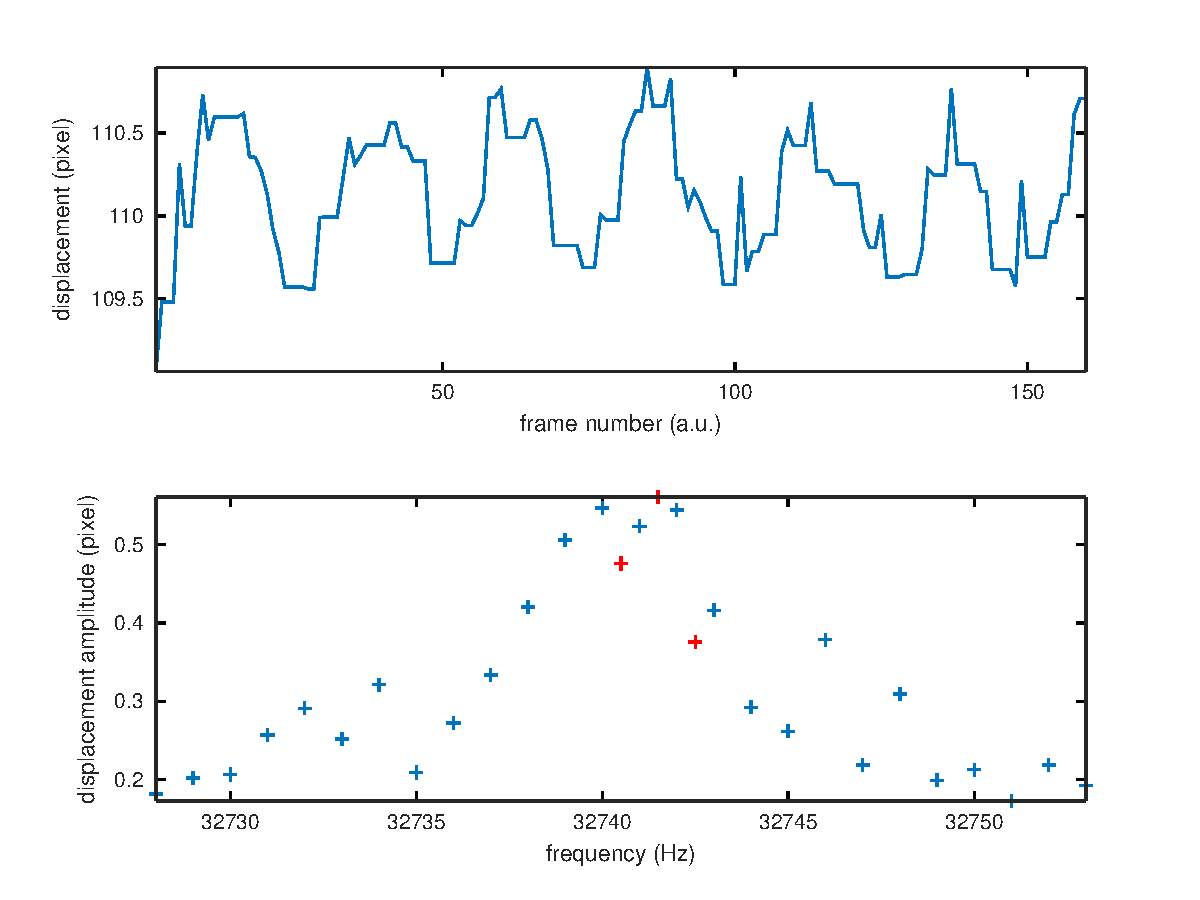
\includegraphics[width=0.49\linewidth]{fonction_de_transfert.pdf}
}
\end{enumerate}
\end{frame}

\begin{frame}[fragile]\frametitle{Meaning of ``super-resolution''}

{\footnotesize
The correlation can detect sub-pixel displacement, as demonstrated here by oversampling the signal
for sub-sampling period displacement\par}

\vspace{0.081cm}
\begin{minipage}[t]{\linewidth}
\begin{minipage}{.50\linewidth}
\lstinputlisting[language=Python,basicstyle=\tiny]{demo_polyfit.py}
\end{minipage}
\begin{minipage}{.49\linewidth}
\vspace{-0.8cm}
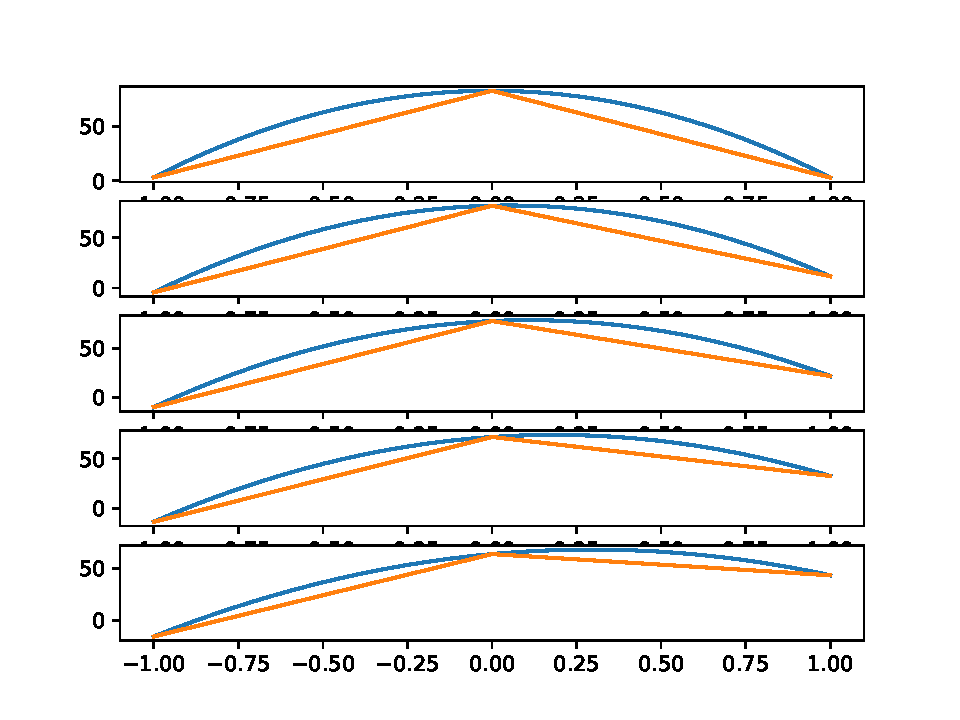
\includegraphics[width=\linewidth]{subpixel.pdf}

\vspace{-0.2cm}
fractional value of the correlation max {\bf position}\\
991.99 ~~ (oversampling by FFT, zero padding \\
992.05 ~~ and iFFT)\\
992.11\\
992.18\\
992.29\\
...

\end{minipage}
\end{minipage}
\end{frame}

\begin{frame}[fragile]\frametitle{For more information ...}

\vspace{-0.1cm}
Tuning fork:
{\footnotesize
\begin{enumerate}
\item T. Hunkin \& R. Garrod, {\em Secret Life Of Machines:
The Quartz Watch} (1991), at \url{https://www.youtube.com/watch?v=nQ9_bOIj49s}
\item M.A. Lombardi, {\em The Evolution of Time Measurement, Part 2: Quartz Clocks},
IEEE Instrumentation \& Measurement Magazine (Oct. 2011), pp.41--
\item J.-M Friedt, \'E. Carry, {\em Introduction au diapason \`a quartz}, Bull. de l'Union des Physiciens {\bf 879} 1137--1146 (2005) [in French]
\item J.-M Friedt, \'E. Carry, {\em Introduction to the quartz tuning fork}, American Journal of 
Physics, pp.415-422 (2007)
\item J.Marc, C. Canard, A. Vailly, V. Pichery, J.-M. Friedt, {\em Le diapason \`a quartz comme 
capteur~: utilisation de la carte son de PC pour l'instrumentation}, Bull. de l'Union des Physiciens {\bf 958}, pp.1051--1073 (2013) [in French]
\item J.-M. Friedt, {\em Mesure stroboscopique du champ de d\'eplacement d'un diapason \`a quartz 
au moyen d'une carte son et d'une webcam}, Bull. de l'Union des Physiciens {\bf 999} (2017) [in French]
\end{enumerate}
}

Stroboscopy:
{\footnotesize
\begin{enumerate}
\item N.S. Gingrich, {\em Stroboscopic Aids in the Teaching of Physics}, American Journal of 
Physics {\bf 5}, 277 (1937)
\item S. Gupta \& B. Jalali, {\em Time stretch enhanced recording oscilloscope}
Appl. Phys. Lett. {\bf 94}, 041105 (2009)
\item J.S. Baskin \& A.H. Zewail, {\em Freezing Atoms in Motion: Principles of 
Femtochemistry and Demonstration by Laser Stroboscopy}, J. Chem. Educ. {\bf 
78} (6), p 737 (2001)
\end{enumerate}
}
\end{frame}

\begin{frame}[fragile]\frametitle{Software for image processing example}

GNU/Octave version\vfill

\begin{lstlisting}[language=Octave,basicstyle=\tiny]
pkg load signal
frequence=[32728:32753]; films=dir('./?????.avi');
for nfilm=1:length(films)
  system('rm -f ./*jpg');
  system(['mplayer -vo jpeg ./',films(nfilm).name]);
  d=dir('./*.jpg');
  x=imread(d(20).name);
%  figure(1);imagesc(x);
  x=x(:,:,1);
  reference=x(440,492:600);
  reference=reference-mean(reference);
  m=1;
  for k=21:180
    x=imread(d(k).name);
    x=x(:,:,1);
    mesure=x(440,492:600); 
    mesure=mesure-mean(mesure);
    xc=xcorr(reference,mesure);
    [a(m),b(nfilm,m)]=max(xc);
    [u,v]=polyfit([b(nfilm,m)-2:b(nfilm,m)+2],xc([b(nfilm,m)-2:b(nfilm,m)+2]),2);
    xi=linspace(b(nfilm,m)-2,b(nfilm,m)+2,1024);
    yi=polyval(u,xi);
    [aa,bb]=max(yi); solution(m,nfilm)=xi(bb);
    m=m+1;
  end
%  figure(2);plot(solution-mean(solution));hold on
  amplitude(nfilm)=std(solution(:,nfilm))
end
\end{lstlisting}
\vfill
Movies at \url{http://jmfriedt.org/TP_diapason.tar.gz}
\end{frame}
\end{document}
